\documentclass[12pt,a4paper]{article}
\usepackage{ctex}
\usepackage{amsmath,amscd,amsbsy,amssymb,latexsym,url,bm,amsthm}
\usepackage{epsfig,graphicx,subfigure}
\usepackage{enumitem,balance}
\usepackage{wrapfig}
\usepackage{mathrsfs,euscript}
\usepackage[usenames]{xcolor}
\usepackage{hyperref}
\usepackage[vlined,ruled,commentsnumbered,linesnumbered]{algorithm2e}
\renewcommand{\algorithmcfname}{算法}
\newtheorem{theorem}{Theorem}
\usepackage{listings}
\newtheorem{lemma}[theorem]{Lemma}
\newtheorem{proposition}[theorem]{Proposition}
\newtheorem{corollary}[theorem]{Corollary}
\newtheorem{exercise}{Exercise}
\newtheorem*{solution}{Solution}
\newtheorem{definition}{Definition}
\theoremstyle{definition}
\definecolor{mygreen}{rgb}{0,0.6,0}
\definecolor{mygray}{rgb}{0.5,0.5,0.5}
\definecolor{mymauve}{rgb}{0.58,0,0.82}
\lstset{
	basicstyle = \footnotesize,       
	breakatwhitespace = false,        
	breaklines = true,                 
	captionpos = b,                    
	commentstyle = \color{mygreen}\bfseries,
	extendedchars = false,   
	keepspaces=true,
	keywordstyle=\color{blue}\bfseries, % keyword style
	language = C++,                     % the language of code
	otherkeywords={string}, 
	numbers=left, 
	numbersep=5pt,
	numberstyle=\tiny\color{mygray},
	rulecolor=\color{black},         
	showspaces=false,  
	showstringspaces=false, 
	showtabs=false,    
	stepnumber=1,         
	stringstyle=\color{mymauve},        % string literal style
	tabsize=2,          
	title=\lstname                      
}
%\numberwithin{equation}{section}
%\numberwithin{figure}{section}

\renewcommand{\thefootnote}{\fnsymbol{footnote}}

\newcommand{\postscript}[2]
{\setlength{\epsfxsize}{#2\hsize}
	\centerline{\epsfbox{#1}}}

\renewcommand{\baselinestretch}{1.0}

\setlength{\oddsidemargin}{-0.365in}
\setlength{\evensidemargin}{-0.365in}
\setlength{\topmargin}{-0.3in}
\setlength{\headheight}{0in}
\setlength{\headsep}{0in}
\setlength{\textheight}{10.1in}
\setlength{\textwidth}{7in}
\makeatletter \renewenvironment{proof}[1][Proof] {\par\pushQED{\qed}\normalfont\topsep6\p@\@plus6\p@\relax\trivlist\item[\hskip\labelsep\bfseries#1\@addpunct{.}]\ignorespaces}{\popQED\endtrivlist\@endpefalse} \makeatother
\makeatletter
\renewenvironment{solution}[1][Solution] {\par\pushQED{\qed}\normalfont\topsep6\p@\@plus6\p@\relax\trivlist\item[\hskip\labelsep\bfseries#1\@addpunct{.}]\ignorespaces}{\popQED\endtrivlist\@endpefalse} \makeatother

\usepackage{listings}

\begin{document}
\noindent

%========================================================================
\noindent\framebox[\linewidth]{\shortstack[c]{
\Large{\textbf{Report}}\vspace{1mm}\\
CS214-Algorithm and Complexity, Spring 2018}}
\begin{center}
\footnotesize{\color{black} Name: 杨培灏  \quad Student ID: 516021910233}
\end{center}

\textbf{问题概述:}判断连连看游戏中两个给定位置是否能够合法相连。

\textbf{输入:}读取in.dat文件,文件格式为
\begin{gather*}
\begin{bmatrix}
x & y\\
\end{bmatrix}\quad\\
\begin{bmatrix}
a_{11}&\cdots&a_{1n}\\
\vdots&\ddots&\vdots\\
a_{n1}&\cdots&a_{nn}\\
\end{bmatrix}\quad\\
\begin{bmatrix}
p & q\\
m & n\\
\end{bmatrix}
\end{gather*}
首行为输入规模,表示x行y列棋盘。之后x行y列矩阵为棋盘上各个位置的情况,用非负数表示棋盘各个位置的情况,0表示没有图案。最后两行$m,n$和$p,q$为给定点坐标。默认可以超出地图。

\begin{enumerate}
	\item{
		\textbf{算法}
		
		在忽略相关规则的简单情况下,即只需要考虑是否存在连通的路径:
		\begin{enumerate}
			\item 直接DFS遍历图寻找两点间是否存在路径
			\item 直接BFS遍历图寻找两点间是否存在路径
		\end{enumerate}
		但是连连看有特殊的规则,两点连接时所经过的路径(连接路径)不能超过两个拐点。加上这个限制条件后,改进的方法为:
		\begin{enumerate}
			\item{
				分类搜索。实现的思路是将问题分解,运用归纳法的思想,如果已经找到了起点A到中转点B的$(n-1)$个拐点的路径,那么只需要找到B到终点C的直线路径,把他们接在一起就得到了从A到C的$n$个拐点的路径。又由于这里拐点数不能超过两个,所以这里的两点间连通实际上只有三种情况:
				\begin{enumerate}
					\item 直线连接。此时A、B两点的横坐标x或纵坐标y是相等的。
					\item 一个拐点。此时A、B两点的横坐标x和纵坐标y是不相等的。此时A、B分别为一个矩形的对角顶点,而矩形的两侧边缘如果存在一边是畅通的,就可以完成一个拐点的连通。
					\item 两个拐点。根据之前的分析,两个拐点的情况可以由两个基本的情况组成,即直线连接,一个拐点连接组成。
				\end{enumerate}
			} 
			
			\item{修改的广度优先搜索。算法的思想是如果能将所有与起点A点经过不多于两个拐点的路径相连的位置全部找出来,加入一个集合S中。由于拐点数不能超过2,所以可以重复两步。那么判断终点B能否与A相连消除,只需要判断B是否属于S即可。
				\begin{center}
					\begin{algorithm}[H]
						\caption{enhencedBFS()}
						\KwIn{起点A,终点B,地图}
						initialize set $S,T=\emptyset$;\\
						S.push(A);\\
						\For{$i=0\to2$}{
							\For{$v \in S$}{
								\For{$u \in v's neighbors$}{
									T.push(u);
								}
							}
							\For{$u \in T$}{
								S.push(u);
							}
						}
					\end{algorithm}
				\end{center}
			}
		\end{enumerate}
	}
	
	\item{
		\textbf{代码}
		几个通用的功能函数
\begin{lstlisting}
void showDFSPath(pair<int, int> now)
{ //path中保留的是后继
	while (now != endPoint)
	{
		cout << now.first << "," << now.second << "->";
		now = path[now.first][now.second];
	}
}
void showBFSPath(pair<int, int> now)
{ //path中保留的是前继
	if (now != pair<int, int>(0, 0))
	{
		showBFSPath(path[now.first][now.second]);
	}
	else return;
	cout << now.first << "," << now.second << "->";
}

void showPath(pathType type)
{
	if (type == BFSpath || type == enhencedBFSpath)
	{
		showBFSPath(path[endPoint.first][endPoint.second]);
		cout << endPoint.first << "," << endPoint.second << endl;
	}
	else if (type == DFSpath || classificationPath)
	{
		showDFSPath(startPoint);
		cout << endPoint.first << "," << endPoint.second << endl;
	}
}
			
void clear()
{
	testTimes = 0;
	for (int i = 0; i < row; ++i)
	{
		for (int j = 0; j <= col + 1; ++j)
		{
			path[i][j] = pair<int, int>(0, 0);
		}
	}
	for (int i = 0; i <= row + 1; ++i)
	{
		for (int j = 0; j <= col + 1; ++j)
		{
			visited[i][j] = false;
		}
	}
}
\end{lstlisting}
		
		接下来是不考虑规则简化问题吼,前两个基础算法的实现:	
		\begin{enumerate}
			\item{
\begin{lstlisting}
bool DFS(int x, int y)
{
	testTimes++;
	visited[x][y] = true;
	if (x == endPoint.first && y == endPoint.second)
	{
		return true;
	}
	else
	{
		if (matrix[x][y] == 0)
		{
			if (x < row + 1 && !visited[x + 1][y])
			{
				if (DFS(x + 1, y))
				{
					path[x][y] = pair<int, int>(x + 1, y);
					return true;
				}
			}
			if (y < col + 1 && !visited[x][y + 1])
			{
				if (DFS(x, y + 1))
				{
					path[x][y] = pair<int, int>(x, y + 1);
					return true;
				}
			}
			if (x > 0 && !visited[x - 1][y])
			{
				if (DFS(x - 1, y))
				{
					path[x][y] = pair<int, int>(x - 1, y);
					return true;
				}
			}
			if (y > 0 && !visited[x][y - 1])
			{
				if (DFS(x, y - 1))
				{
					path[x][y] = pair<int, int>(x, y - 1);
					return true;
				}
			}
		}
		return false;
	}
}
						
bool DFS()
{
	clear();
	visited[startPoint.first][startPoint.second] = true;
	if (startPoint.first < row + 1)
	{
		if (DFS(startPoint.first + 1, startPoint.second))
		{
		path[startPoint.first][startPoint.second] = pair<int, int>(startPoint.first + 1, startPoint.second);
		return true;
		}
	}
	if (startPoint.second < col + 1)
	{
		if (DFS(startPoint.first, startPoint.second + 1))
		{
			path[startPoint.first][startPoint.second] = pair<int, int>(startPoint.first, startPoint.second + 1);
			return true;
		}
	}
	if (startPoint.first > 0)
	{
		if (DFS(startPoint.first - 1, startPoint.second))
		{
			path[startPoint.first][startPoint.second] = pair<int, int>(startPoint.first - 1, startPoint.second);
			return true;
		}
	}
	if (startPoint.second > 0)
	{
		if (DFS(startPoint.first, startPoint.second - 1))
		{
			path[startPoint.first][startPoint.second] = pair<int, int>(startPoint.first, startPoint.second - 1);
			return true;
		}
	}
	return false;
}
				\end{lstlisting} 
			}
			\item{
\begin{lstlisting}
bool BFS(int x, int y)
{
	pair<int, int> child;
	BFSqueue.push(pair<int, int>(x, y));
	while (!BFSqueue.empty())
	{
		child = BFSqueue.front();
		BFSqueue.pop();
		visited[child.first][child.second] = true;
		testTimes++;
		if (child.first == endPoint.first && child.second == endPoint.second)
		{
			return true;
		}
		if (matrix[child.first][child.second] == 0)
		{
			if (child.first < row + 1 && !visited[child.first + 1][child.second])
			{
				BFSqueue.push(pair<int, int>(child.first + 1, child.second));
				path[child.first + 1][child.second] = child;
			}
			if (child.second < col + 1 && !visited[child.first][child.second + 1])
			{
				BFSqueue.push(pair<int, int>(child.first, child.second + 1));
				path[child.first][child.second + 1] = child;
			}
			if (child.first > 0 && !visited[child.first - 1][child.second])
			{
				BFSqueue.push(pair<int, int>(child.first - 1, child.second));
				path[child.first - 1][child.second] = child;
			}
			if (child.second > 0 && !visited[child.first][child.second - 1])
			{
				BFSqueue.push(pair<int, int>(child.first, child.second - 1));
				path[child.first][child.second - 1] = child;
			}
		}
	}
	return false;
}
				
bool BFS()
{
	clear();
	visited[startPoint.first][startPoint.second] = true;
	if (startPoint.first < row + 1)
	{
		if (BFS(startPoint.first + 1, startPoint.second))
		{
			path[startPoint.first + 1][startPoint.second] = pair<int, int>(startPoint.first, startPoint.second);
			return true;
		}
	}
	if (startPoint.second < col + 1)
	{
		if (BFS(startPoint.first, startPoint.second + 1))
		{
			path[startPoint.first][startPoint.second + 1] = pair<int, int>(startPoint.first, startPoint.second);
			return true;
		}
	}
	if (startPoint.first > 0)
	{
		if (BFS(startPoint.first - 1, startPoint.second))
		{
			path[startPoint.first - 1][startPoint.second] = pair<int, int>(startPoint.first, startPoint.second);
			return true;
		}
	}
	if (startPoint.second > 0)
	{
		if (BFS(startPoint.first, startPoint.second - 1))
		{
			path[startPoint.first][startPoint.second - 1] = pair<int, int>(startPoint.first, startPoint.second);
			return true;
		}
	}
	return false;
}
\end{lstlisting}
			}
		\end{enumerate}
		在了解规则后,完整的代码如下:
		\begin{enumerate}
			\item{
\begin{lstlisting}
bool enhencedBFS()
{ //使用两个临时的集合进行遍历,确定可以到达后存储进稳定的集合
	clear();
	visited[startPoint.first][startPoint.second] = true;
	templinkedPoints.insert(pair<int, int>(startPoint.first, startPoint.second));
	for (int loopTimes = 0; loopTimes < 3; ++loopTimes)
	{
		for (set<pair<int, int>>::iterator it = templinkedPoints.begin(); it != templinkedPoints.end(); ++it)
		{
			int i = 1;
			while ((*it).first + i < row + 1 && !visited[(*it).first + i][(*it).second] && matrix[(*it).first + i][(*it).second] == 0)
			{
				tempStorePoints.insert(pair<int, int>((*it).first + i, (*it).second));
				path[(*it).first + i][(*it).second] = *it;
				visited[(*it).first + i][(*it).second] = true;
				++i;
				++testTimes;
			}
			//上方while遍历某个方向上的通路,停止后遇到的第一个阻塞无法加入临时集合,应该加入稳定集合
			if ((*it).first + i < row + 1 && matrix[(*it).first + i][(*it).second] != 0)
			{
				linkedPoints.insert(pair<int, int>((*it).first + i, (*it).second));
				path[(*it).first + i][(*it).second] = *it;
				visited[(*it).first + i][(*it).second] = true;
			}
								
			i = 1;
			while ((*it).second + i < col + 1 && !visited[(*it).first][(*it).second + i] && matrix[(*it).first][(*it).second + i] == 0)
			{
				tempStorePoints.insert(pair<int, int>((*it).first, (*it).second + i));
				path[(*it).first][(*it).second + i] = *it;
				visited[(*it).first][(*it).second + i] = true;
				++i;
				++testTimes;
			}
			if ((*it).second + i < col + 1 && matrix[(*it).first][(*it).second + i] != 0)
			{
				linkedPoints.insert(pair<int, int>((*it).first, (*it).second + i));
				path[(*it).first][(*it).second + i] = *it;
				visited[(*it).first][(*it).second + i] = true;
			}
								
			i = 1;
			while ((*it).first - i > 0 && !visited[(*it).first - i][(*it).second] && matrix[(*it).first - i][(*it).second] == 0)
			{
				tempStorePoints.insert(pair<int, int>((*it).first - i, (*it).second));
				path[(*it).first - i][(*it).second] = *it;
				visited[(*it).first - i][(*it).second] = true;
				++i;
				++testTimes;
			}
			if ((*it).first - i > 0 && matrix[(*it).first - i][(*it).second] != 0)
			{
				linkedPoints.insert(pair<int, int>((*it).first - i, (*it).second));
				path[(*it).first - i][(*it).second] = *it;
				visited[(*it).first - i][(*it).second] = true;
			}
								
			i = 1;
			while ((*it).second - i > 0 && !visited[(*it).first][(*it).second - i] && matrix[(*it).first][(*it).second - i] == 0)
			{
				tempStorePoints.insert(pair<int, int>((*it).first, (*it).second - i));
				path[(*it).first][(*it).second - i] = *it;
				visited[(*it).first][(*it).second - i] = true;
				++i;
				++testTimes;
			}
			if ((*it).second - i > 0 && matrix[(*it).first][(*it).second - i] != 0)
			{
				linkedPoints.insert(pair<int, int>((*it).first, (*it).second - i));
				path[(*it).first][(*it).second - i] = *it;
				visited[(*it).first][(*it).second - i] = true;
			}
		}
		templinkedPoints.clear();
		for (set<pair<int, int>>::iterator it = tempStorePoints.begin(); it != tempStorePoints.end(); ++it)
		{
			templinkedPoints.insert(*it);
		}
		tempStorePoints.clear();
		for (set<pair<int, int>>::iterator it = templinkedPoints.begin(); it != templinkedPoints.end(); ++it)
		{
			linkedPoints.insert(*it);
		}
		if (linkedPoints.find(endPoint) != linkedPoints.end())
		{
			path[startPoint.first][startPoint.second] = pair<int, int>(0, 0);
			testTimes = linkedPoints.size();
			return true;
		}
	}
	testTimes = linkedPoints.size();
	path[startPoint.first][startPoint.second] = pair<int, int>(0, 0);
	return linkedPoints.find(endPoint) != linkedPoints.end();
}
				\end{lstlisting}
			} 
			\item{
\begin{lstlisting}
bool straightLinked(pair<int, int> startNow, pair<int, int> endNow)
{ //直接相连
	testTimes++;
	if (startNow.first == endNow.first)
	{
		for (int i = min(startNow.second, endNow.second) + 1; i <= max(startNow.second, endNow.second) - 1; ++i)
		{
			if (matrix[startNow.first][i] != 0)	return false;
		}
		path[startNow.first][startNow.second] = endNow;
		return true;
	}
	else if (startNow.second == endNow.second)
	{
		for (int i = min(startNow.first, endNow.first) + 1; i <= max(startNow.first, endNow.first) - 1; ++i)
		{
			if (matrix[i][startNow.second] != 0) return false;
		}
		path[startNow.first][startNow.second] = endNow;
		return true;
	}
	else return false;
}

bool oneTurnLinked(pair<int, int> startNow, pair<int, int> endNow)
{ //一拐点相连
	testTimes++;
	if (startNow.first != endNow.first && startNow.second != endNow.second)
	{
		if (matrix[startNow.first][endNow.second] == 0)
		{
			if (straightLinked(startNow, pair<int, int>(startNow.first, endNow.second)) && straightLinked(pair<int, int>(startNow.first, endNow.second), endNow))
			{
				return true;
			}
		}
		if (matrix[endNow.first][startNow.second] == 0)
		{
			if (straightLinked(startNow, pair<int, int>(endNow.first, startNow.second)) && straightLinked(pair<int, int>(endNow.first, startNow.second), endNow))
			{
				return true;
			}
		}
	}
	return false;
}
bool twoTurnLinked(pair<int, int> startNow, pair<int, int> endNow)
{ //两拐点相连
	testTimes++;
	if (startNow.first == endNow.first)
	{
		for (int i = 0; i <= row + 1; ++i)
		{
			if (i == startNow.first) continue;
			if (straightLinked(startNow, pair<int, int>(i, startNow.second)) && oneTurnLinked(pair<int, int>(i, startNow.second), endNow))
			{
				return true;
			}
		}
	}
	else if (startNow.second == endNow.second)
	{
		for (int i = 0; i <= col + 1; ++i)
		{
			if (i == startNow.second)continue;
			if (straightLinked(startNow, pair<int, int>(startNow.first, i)) && oneTurnLinked(pair<int, int>(startNow.first, i), endNow))
			{
				return true;
			}
		}
	}
	return false;
}

bool classification()
{
	clear();
	visited[startPoint.first][startPoint.second] = true;
	return straightLinked(startPoint, endPoint) || oneTurnLinked(startPoint, endPoint) || twoTurnLinked(startPoint, endPoint);
}
\end{lstlisting}
			}
		\end{enumerate}
	}

	\item{
		\textbf{测试}
		
		测试文件如下
\begin{lstlisting}
#include <iostream>
#include <string>
#include <ctime>
#include <queue>
#include <set>
#include <utility>
#include <algorithm>
#pragma warning(disable : 4996)
using namespace std;
	
enum pathType
{
	DFSpath,
	BFSpath,
	enhencedBFSpath,
	classificationPath
};
		
const string answer[2] = { "不存在路径,无法消除", "存在路径可以消除" };
pair<int, int> startPoint, endPoint;
int **matrix;
bool **visited;
pair<int, int> **path;
int row, col;
int testTimes;
queue<pair<int, int>> BFSqueue;
set<pair<int, int>> linkedPoints, tempStorePoints, templinkedPoints;
int main()
{
	bool answerIndex = false;
	freopen("test.txt", "r", stdin);
	cin >> row >> col;
	matrix = new int *[row + 2];
	for (int i = 0; i < row + 2; ++i)
	{
		matrix[i] = new int[col + 2];
	}
	visited = new bool *[row + 2];
	for (int i = 0; i < row + 2; ++i)
	{
		visited[i] = new bool[col + 2];
	}
	path = new pair<int, int> *[row + 2];
	for (int i = 0; i < row + 2; ++i)
	{
		path[i] = new pair<int, int>[col + 2];
	}
	for (int i = 0; i < row + 2; ++i)
	{
		matrix[i][0] = 0;
		matrix[i][col + 1] = 0;
	}
	for (int i = 0; i < col + 2; ++i)
	{
		matrix[0][i] = 0;
		matrix[row + 1][i] = 0;
	}
	for (int i = 1; i <= row; ++i)
	{
		for (int j = 1; j <= col; ++j)
		{
			cin >> matrix[i][j];
		}
	}
	for (int i = 0; i <= row + 1; ++i)
	{
		for (int j = 0; j <= col + 1; ++j)
		{
			cout << matrix[i][j] << " ";
		}
		cout << endl;
	}
	cin >> startPoint.first >> startPoint.second >> endPoint.first >> endPoint.second;
	cout << "杨培灏516021910233" << endl;
	if (matrix[startPoint.first][startPoint.second] !=  matrix[endPoint.first][endPoint.second])
	{
		cout << "图形不同不可能消除" << endl;
	}
	else
	{
		answerIndex = DFS();
		cout << "DFS方法" << answer[answerIndex];
		if (answerIndex)
		{
			cout << "测试次数:" << testTimes << endl << "路径:";
			showPath(DFSpath);
		}
		answerIndex = BFS();
		cout << "BFS方法" << answer[answerIndex];
		if (answerIndex)
		{
			cout << "测试次数:" << testTimes << endl << "路径:";
			showPath(BFSpath);
		}
		answerIndex = enhencedBFS();
		cout << "BFS增强方法" << answer[answerIndex];
		if (answerIndex)
		{
			cout << "测试次数:" << testTimes << endl << "路径:";
			showPath(enhencedBFSpath);
		}
		answerIndex = classification();
		cout << "分类方法" << answer[answerIndex];
		if (answerIndex)
		{
			cout << "测试次数:" << testTimes << endl << "路径:";
			showPath(classificationPath);
		}
	}
	return 0;
}
		\end{lstlisting}
		
		地图输入见下图,为$7\times 7$的地图,处理时补充成了$9\times 9$的地图。测试点为$(1,1)$和$(3,1)$。测试结果输出如下:
		\begin{center}
			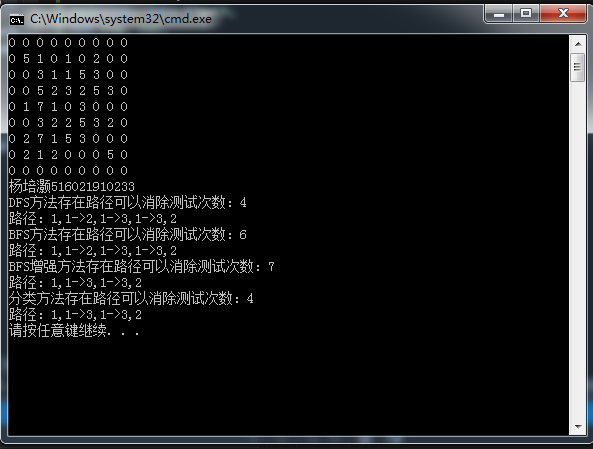
\includegraphics[width=0.75\textwidth]{test.png}
		\end{center}
		
	} 
	
	\item{
		\textbf{讨论}
		
		在不考虑规则的简单情况下,直接遍历寻找连通路径即可。最坏情况遍历整个地图矩阵,时间复杂度为$\mathcal{O}(|V|^2)$。之后的加入游戏规则的算法,最坏情况也会遍历所有的点,时间复杂度和解决简单之前问题相同,为$\mathcal{O}(|V|^2)$。
	}
\end{enumerate}
%========================================================================
\end{document}
